\documentclass{article}
\usepackage[utf8]{inputenc}

\usepackage{tikz}
\usetikzlibrary{positioning}

\begin{document}

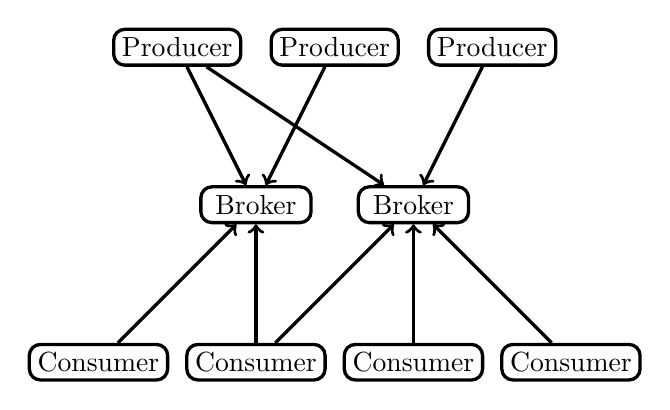
\begin{tikzpicture}[ % has a lot of options; consult the pgf manual
bend angle=45,
long_square/.style={rectangle, draw=black, fill=white, very thick, inner sep=3pt, minimum width=14mm},
rounded_square/.style={rectangle, rounded corners, draw=black, fill=white, very thick, inner sep=3pt, minimum width=14mm},
circle/.style={rectangle, rounded corners=2mm, draw=black, fill=white, very thick, minimum size=4mm},
both_arrow/.style={<->, very thick},
out_arrow/.style={->, very thick},
in_arrow/.style={<-, very thick},
above_edge_text/.style={above, midway, sloped}
]

% \node[type](name_of_node)[above/below/right/left/...=of name_of_node]{node_text}
%   edge[<->, bend left/right] node[auto, swap]{edge_text}(out_name_of_node)
% OR
% \node[type](name_of_node)[above/below/right/left/...=of name_of_node]{node_text}
\node[rounded_square](prod_1) at (1,0) {Producer};
\node[rounded_square](prod_2) at (3,0) {Producer};
\node[rounded_square](prod_3) at (5,0) {Producer};

\node[rounded_square](broker_1) at (2,-2) {Broker};
\node[rounded_square](broker_2) at (4,-2) {Broker};

\node[rounded_square](cons_1) at (0,-4) {Consumer};
\node[rounded_square](cons_2) at (2,-4) {Consumer};
\node[rounded_square](cons_3) at (4,-4) {Consumer};
\node[rounded_square](cons_4) at (6,-4) {Consumer};


% \draw[->](name_of_node.direction) -- (name_of_node.direction)
% OR
% \draw[->](name_of_node.direction) to [bend right] node[]{edge_text} (name_of_node.direction)
% OR
% \draw[->](name_of_node.direction) .. controls +(up/down/right/left:10mm) and +(up/down/right/left:10mm) .. (name_of_node.direction);
\draw[out_arrow](prod_1) to [] node[auto]{} (broker_1);
\draw[out_arrow](prod_1) to [] node[auto]{} (broker_2);
\draw[out_arrow](prod_2) to [] node[auto]{} (broker_1);
\draw[out_arrow](prod_3) to [] node[auto]{} (broker_2);

\draw[out_arrow](cons_1) to [] node[auto]{} (broker_1);
\draw[out_arrow](cons_2) to [] node[auto]{} (broker_1);
\draw[out_arrow](cons_2) to [] node[auto]{} (broker_2);
\draw[out_arrow](cons_3) to [] node[auto]{} (broker_2);
\draw[out_arrow](cons_4) to [] node[auto]{} (broker_2);

\end{tikzpicture}

\end{document}